%%%%%%%%%%%%%%%%%%%%%%%%%%%%%%%%%%%%%%%%%
% baposter Portrait Poster
% LaTeX Template
% Version 1.0 (15/5/13)
%
% Created by:
% Brian Amberg (baposter@brian-amberg.de)
%
% This template has been downloaded from:
% http://www.LaTeXTemplates.com
%
% License:
% CC BY-NC-SA 3.0 (http://creativecommons.org/licenses/by-nc-sa/3.0/)
%
%%%%%%%%%%%%%%%%%%%%%%%%%%%%%%%%%%%%%%%%%

%----------------------------------------------------------------------------------------
%	PACKAGES AND OTHER DOCUMENT CONFIGURATIONS
%----------------------------------------------------------------------------------------

\documentclass[a0paper,portrait]{baposter}

\usepackage[T1]{fontenc}
\usepackage[english,russian]{babel}
\usepackage[utf8]{inputenc}
\usepackage{type1ec}
\usepackage{amsmath,mathrsfs,mathtext}
\usepackage{graphicx, epsfig}
\RequirePackage{array}
\usepackage{latexsym}
\RequirePackage{amssymb}
\RequirePackage{amsmath}
\RequirePackage{mathrsfs}



\usepackage[font=small,labelfont=bf]{caption} % Required for specifying captions to tables and figures
\usepackage{booktabs} % Horizontal rules in tables
\usepackage{relsize} % Used for making text smaller in some places

\graphicspath{{figures/}} % Directory in which figures are stored

\definecolor{bordercol}{RGB}{40,40,40} % Border color of content boxes
\definecolor{headercol1}{RGB}{230,230,230} % Background color for the header in the content boxes (left side)
\definecolor{headercol2}{RGB}{230,230,230} % Background color for the header in the content boxes (right side)
\definecolor{headerfontcol}{RGB}{0,0,0} % Text color for the header text in the content boxes
\definecolor{boxcolor}{RGB}{255,255,255} % Background color for the content in the content boxes

\newcommand{\x}{\mathbf{x}}
\newcommand{\h}{\mathbf{h}}
\newcommand{\w}{\mathbf{w}}
\newcommand{\W}{\mathbf{W}}
\newcommand{\y}{\mathbf{y}}
\newcommand{\X}{\mathbf{X}}
\newcommand{\Y}{\mathbf{Y}}
\newcommand{\fx}{\mathbf{f}}
\newcommand{\fs}{\mbox{f}}

\newcommand\myop[1]{\mathop{\operator@font #1}\nolimits}
\newcommand\mylim[1]{\mathop{\operator@font #1}\limits}

\newcommand\argmin{\mylim{arg\,min}}
\newcommand\argmax{\mylim{arg\,max}}

\begin{document}

\background{ % Set the background to an image (background.pdf)
%\begin{tikzpicture}[remember picture,overlay]
%\draw (current page.north west)+(-2em,2em) node[anchor=north west]
%{\includegraphics[height=1.1\textheight]{background}};
%\end{tikzpicture}
}

\begin{poster}{
grid=false,
borderColor=bordercol, % Border color of content boxes
headerColorOne=headercol1, % Background color for the header in the content boxes (left side)
headerColorTwo=headercol2, % Background color for the header in the content boxes (right side)
headerFontColor=headerfontcol, % Text color for the header text in the content boxes
boxColorOne=boxcolor, % Background color for the content in the content boxes
headershape=roundedright, % Specify the rounded corner in the content box headers
headerfont=\Large\sf\bf, % Font modifiers for the text in the content box headers
textborder=rectangle,
background=user,
headerborder=open, % Change to closed for a line under the content box headers
boxshade=plain
}
{}
%
%----------------------------------------------------------------------------------------
%	TITLE AND AUTHOR NAME
%----------------------------------------------------------------------------------------
%
{\sf\bf Вероятностный подход для задачи предсказания биологической активности ядерных рецепторов} % Poster title
{\vspace{1em} Володин~С.\,Е., Попова~М., Стрижов~В.\,В.\\ % Author names
{\smaller sergei.volodin@phystech.edu, maria\_popova@phystech.edu, strijov@ccas.ru}} % Author email addresses
%{\includegraphics[scale=0.15]{logo}} % University/lab logo

%----------------------------------------------------------------------------------------
%	INTRODUCTION
%----------------------------------------------------------------------------------------

\headerbox{Цель исследования}{name=introduction,column=0,row=0}{

Предсказание взаимодействия двух типов молекул: лиганд и рецепторов. Задача является важной для разработки различных лекарств. Из-за нехватки данных биохимическое моделирование \cite{Myint2012} неприменимо.

{\bf Проблема}

	События реакции лиганда с различными рецепторами не независимы. Классификатор, не учитывающий их, имеет неоптимальный результат. \cite{popova1}

{\bf Задача}

	Необходимо построить
	\begin{enumerate}
		\item вероятностную модель, учитывающую зависимости
		\item бинарный классификатор
	\end{enumerate}
%-------------------------------------------------------
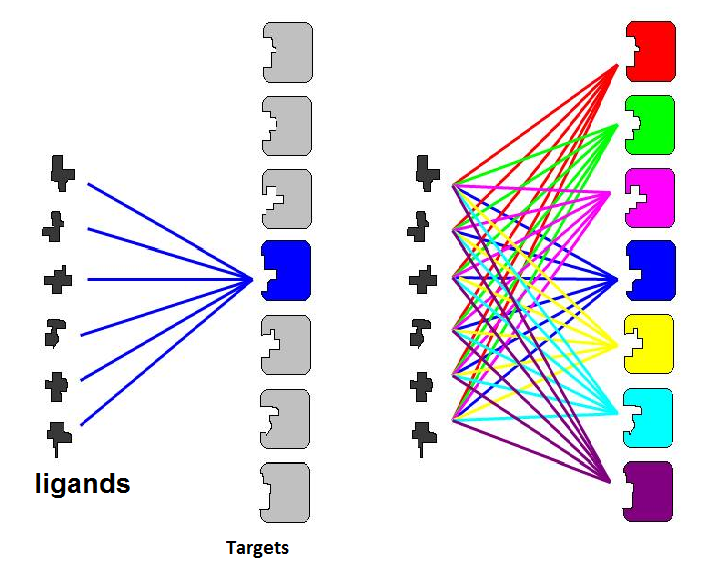
\includegraphics{dependence}
}

%----------------------------------------------------------------------------------------
%	MATERIALS AND METHODS
%----------------------------------------------------------------------------------------

\headerbox{Постановка задачи}{name=methods,column=0,below=introduction}{
Задана выборка $\mathfrak{D}=\{(\x_i,\y_i)\}=\mathfrak{L}\sqcup\mathfrak{T}$.

$\x_i\in \mathbb{R}^n$. $\y_i\in \{0,1,\Box\}^l$ (задача класса MLC) %, $\Box$~--- пропуск в данных.

$\X, \Y$~--- случайные величины %, между классами есть зависимости.

{\bf 1. Восстановление плотности}

$\fs(\x,\y|\w)=P(\Y=\y|\X=\x;\w)$~--- модель классификации.

Максимизируется правдоподобие выборки:

%Функция потерь~--- логарифм правдоподобия
%$$Q(\fs|\w, \mathcal{Z})=-\sum_{(\x,\y)\in\mathcal{Z}}\log %\fs(\w,\x,\y)P(\X=\x)$$

%	Требуется минимизировать $Q$:
$$\w^*=\underset{{\w\in\W}}{\arg\max}\ln Q(\fs|\w,\mathfrak{L})$$
 
{\bf 2. Бинарный классификатор}

$L(\y,\y')$~--- функция потерь

$$h(x)=\underset{\y\in \Y}{\arg\min}\,\mathbb{E}_{\Y|\X=\x}L(\Y,\y)$$

}

%----------------------------------------------------------------------------------------
%	CONCLUSION
%----------------------------------------------------------------------------------------

\headerbox{Восстановление плотности}{name=conclusion,column=0,below=methods,above=bottom}{
Probabilistic Classifier Chains \cite{weiwei2010}
\begin{enumerate}
	\item Выразим искомую величину $P(\y|\x)$: $$P(\y|\x)=P(y_1|\x)\prod_{i=2}^lP(y_i|y_1,...,y_{i-1}, \x)$$
	
	\item Задача распадается на $n$ задач поиска $$P(y_1|\x),\,P(y_2|y_1,\x)...,\,P(y_l|y_1,...,y_{l-1},\x)$$
	
	\item Каждую оцениваем при помощи логистической регрессии.
	
	\item Признаки для $i$-й: $\x$, \bf{а также $y_1,...,y_{i-1}$}
\end{enumerate}
}

%----------------------------------------------------------------------------------------
%	REFERENCES
%----------------------------------------------------------------------------------------

%----------------------------------------------------------------------------------------
%	ACKNOWLEDGEMENTS
%----------------------------------------------------------------------------------------


\headerbox{Бинарный классификатор}{name=results1,span=1,column=1,row=0}{ % To reduce this block to 1 column width, remove 'span=2'
Байесовское решающее правило:
$$h(x)=\underset{\y\in \Y}{\arg\min}\,\mathbb{E}_{\Y|\X=\x}L(\Y,\y)$$
Все зависит от $L(\y,\y')$. Какая лучше? \cite{Kr_presentation}
\begin{enumerate}
	\item Hamming Loss: $L(\y,\y')=\sum\limits_{i=1}^l[y_i\neq y'_i]$.\\ $h(x)$ не учитывает зависимости!
	\item Subset Loss: $L(\y,\y')=[\y\neq\y']$
	\item $L(\y,\y')=q(\sum\limits_{i=1}^l[y_i\neq y'_i])$
\end{enumerate}

Решения для разных существенно различны.

%	\centering\medskip%\tabcolsep=2pt%\small
	\begin{tabular}{lrrrr}
		$y_1$ & $y_2$ & $y_3$ & $y_4$ & $P(\y)$\\
		$0$ & $0$ & $0$ & $0$ & $0.30$\\
		$0$ & $1$ & $1$ & $1$ & $0.17$\\
		$1$ & $0$ & $1$ & $1$ & $0.18$\\
		$1$ & $1$ & $0$ & $1$ & $0.17$\\
		$1$ & $1$ & $1$ & $0$ & $0.18$\\
	\end{tabular}



Лучший по Subset Loss: $(0, 0, 0, 0)$

Лучший по Hamming Loss: $(1, 1, 1, 1)$

}

%----------------------------------------------------------------------------------------
%	RESULTS 2
%----------------------------------------------------------------------------------------

\headerbox{Модельные данные}{name=results2,span=1,column=1,below=results1}{ % To reduce this block to 1 column width, remove 'span=2'
	
	1 признак, $l=3$ класса. Плотность:
	
	
	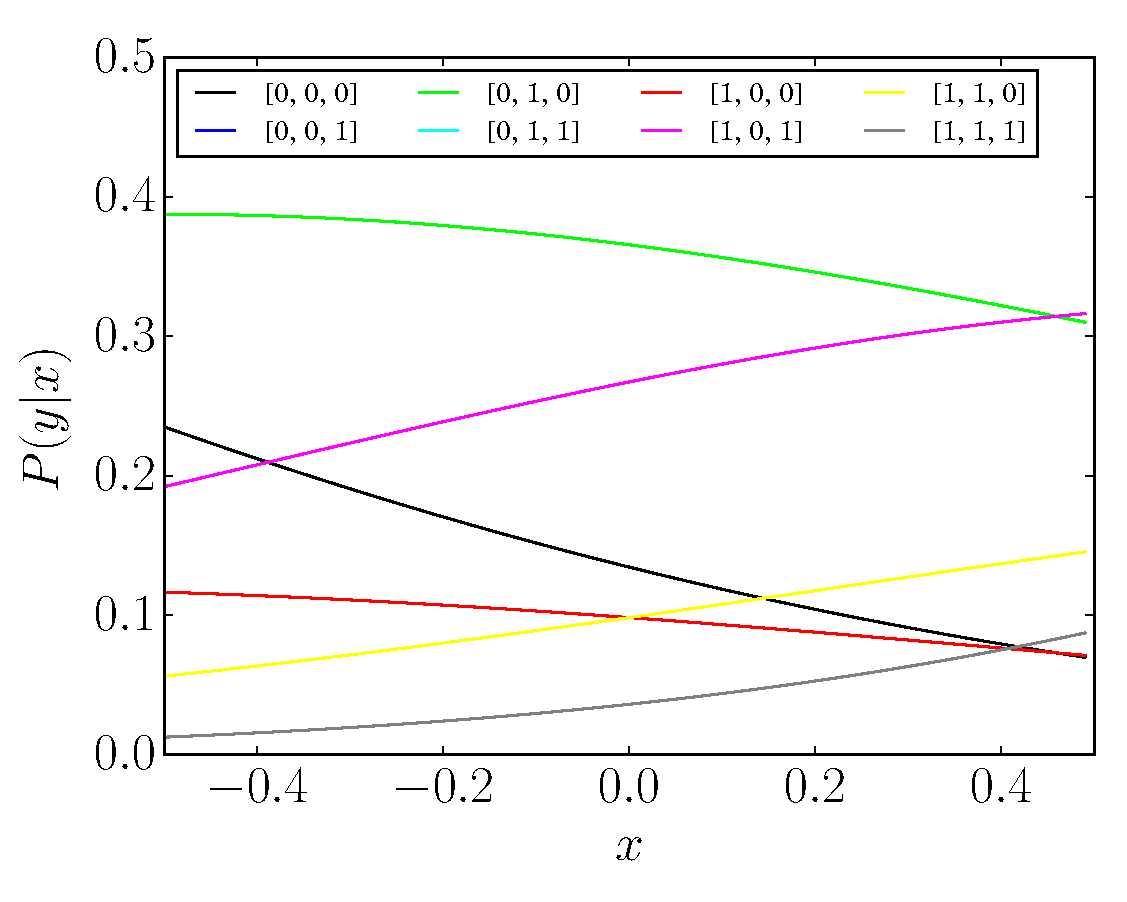
\includegraphics[width=1.0\textwidth]{ModelData}
	
Модели:
\begin{enumerate}
	\item PCC + решающее правило
	\item Binary Relevance~--- l лог. регрессий
\end{enumerate}

Результаты:
\begin{enumerate}	
\item Есть улучшение по Subset Loss
\item Нет улучшений по Hamming Loss
\item Нет улучшений по метрикам отдельных классов	
\end{enumerate}
}

\headerbox{Вычислительный эксперимент}{name=results2,span=2,column=1,below=results2, above=bottom}{

Использованы модельные данные, BR, PCC с различными $L(\y,\y')$

	\begin{tabular}{lrrrr}
		%		\hline
		Метрика &             BR &         PCC (H) &         PCC (M) &         PCC (S) \\
		Hamming     &  0.37 $\pm$ 0.009 &  0.36 $\pm$ 0.02 &  0.36 $\pm$ 0.02 &  0.38 $\pm$ 0.04 \\
		Hamming 1   &   0.31 $\pm$ 0.03 &  0.31 $\pm$ 0.03 &  0.31 $\pm$ 0.02 &  0.31 $\pm$ 0.05 \\
		Hamming 2   &   0.45 $\pm$ 0.04 &  0.45 $\pm$ 0.04 &  0.45 $\pm$ 0.03 &  0.49 $\pm$ 0.05 \\
		Hamming 3   &   0.34 $\pm$ 0.03 &   0.3 $\pm$ 0.03 &  0.31 $\pm$ 0.04 &  0.34 $\pm$ 0.03 \\
		Precision 1   &    0.7 $\pm$ 0.06 &   0.7 $\pm$ 0.06 &  0.73 $\pm$ 0.05 &  0.64 $\pm$ 0.05 \\
		Precision 2   &   0.55 $\pm$ 0.04 &  0.51 $\pm$ 0.01 &  0.47 $\pm$ 0.04 &  0.46 $\pm$ 0.07 \\
		Precision 3   &    0.7 $\pm$ 0.06 &  0.56 $\pm$ 0.05 &    0.5 $\pm$ 0.1 &  0.66 $\pm$ 0.05 \\
		Recall 1   &   0.68 $\pm$ 0.04 &  0.68 $\pm$ 0.04 &  0.68 $\pm$ 0.03 &  0.71 $\pm$ 0.05 \\
		Recall 2   &    0.52 $\pm$ 0.1 &   0.53 $\pm$ 0.1 &  0.54 $\pm$ 0.09 &  0.48 $\pm$ 0.05 \\
		Recall 3   &    0.48 $\pm$ 0.1 &  0.53 $\pm$ 0.06 &  0.52 $\pm$ 0.07 &  0.49 $\pm$ 0.09 \\
		\bf{Subset}     &   0.78 $\pm$ 0.03 &  0.77 $\pm$ 0.05 &  0.77 $\pm$ 0.05 &  0.62 $\pm$ 0.06 \\
		%	\hline
	\end{tabular}
}

\headerbox{Реальные данные}{name=results3,span=1,column=2,row=0}{ % To reduce this block to 1 column width, remove 'span=2'
	Взаимодействие лиганд и рецепторов. Признаки сгенерированы программой биохимической симуляции, ответы~--- результаты экспериментов.
	\begin{enumerate}
		\item 165 признаков, 8000 объектов
		\item 12 классов (рецепторов), используется 3.
		\item Высокая мультиколлинеарность
	\end{enumerate}
	В ответах имеется большое количество пропусков.
	
Результаты:
\begin{enumerate}	
	\item Небольшое улучшение по Subset Loss
	\item Нет улучшений по Hamming Loss
	\item Нет улучшений по метрикам отдельных классов
	
\end{enumerate}
}

\headerbox{Результаты}{name=conclusion,span=1,column=2,below=results3}{ % To reduce this block to 1 column width, remove 'span=2'
		\begin{enumerate}
			\item Предложена модель для предсказания взаимодействия, учитывающая зависимости между классами
			\item Проведено сравнение модели с базовой
			\item PCC лучше BR по метрике Subset Loss
			\item Нет улучшений по отдельным классам
		\end{enumerate}
}
\headerbox{Дальнейшее развитие}{name=plans,span=1,column=2,below=conclusion}{ % To reduce this
		\begin{enumerate}
			\item Улучшение показателей по классам
			\item Замена логистической регрессии на лучший алгоритм
			\item Вычисление для всей выборки
		\end{enumerate}	
}

\headerbox{Список литературы}{name=references,column=2,below=plans}{
	
	\smaller % Reduce the font size in this block
	\renewcommand{\section}[2]{\vskip 0.05em} % Get rid of the default "References" section title
	%	\nocite{*} % Insert publ\textsl{}ications even if they are not cited in the poster
	
	\bibliographystyle{unsrt}
	\bibliography{Volodin2016ProbabilisticReceptorPredictionPoster} % Use sample.bib as the bibliography file
}

%----------------------------------------------------------------------------------------

\end{poster}

\end{document}